	\documentclass[notitlepage, 11pt]{report}
	\usepackage[utf8]{inputenc}
	\usepackage{titling}
	\usepackage{amsmath}
	\usepackage{relsize}
	\usepackage{breqn}
	\usepackage{graphicx}
	\graphicspath{ {./images/} }
	\setlength{\droptitle}{-5em}   % This is your set screw
	\usepackage[a4paper, total={7in, 10in}]{geometry}
	\title{Report \\
		\large{SPS Coursework: An Unknown Signal} \\
	}

	\author{Emil Centiu, zl18810}
	\begin{document}
		
		\maketitle	
		\renewcommand{\thesection}{\arabic{section}}

		\section{Least Squares Regression}
		
		\paragraph*{}	
		Because we can't assume anything about the random error term (i.e. follows a normal distribution like in MLE), Least squares was the go-to method to find the best fitting line. 
		
		The goal is to deterministicaly minimise the sum of squared differences between the observed value of the dependent variable ($ y_{i} $) and the predicted value of the dependent variable ($ \hat{y} $), that is provided by the regression function. In other words, we need to find $a, b$ such that the residual error $R(a, b)$ is minimised, where
		
		\begin{equation*}
			R(a, b) = \sum_{i=1}^{N}(\hat{y_{i}} - y_{i})^2 = 	\sum_{i=1}^{N}((a + bx_i) - y_i)^2
		\end{equation*}
		
		We can observe that $ R(a, b) $ plots as an eliptic paraboloid, so there is only one critical point, and according to Fermat's Theorem, it is a local extreme, hence the minimum value of the function. To find the pair $(a, b)$, we can just calculate the critical point drom the partial derivatives with respect to each variable:
		
		\begin{equation*}
			\dfrac{\delta{} R}{\delta{} a} = 	\dfrac{\delta{}}{\delta{} a} \sum_{i=1}^{N}(y_i^2 + a^2 + 2abx_i + b^2x^2 - 2y_ia - 2y_ibx_i)^2
			= \sum_{i=1}^{N}(2a + 2bx_i - 2y_i) = -2\sum_{i=1}^{N}(y_i - (a+bx_i)) = 0
		\end{equation*}
		\begin{equation*}
			\dfrac{\delta{} R}{\delta{} b} =\dfrac{\delta{}}{\delta{} b} \sum_{i=1}^{N}(y_i^2 + a^2 + 2abx_i + b^2x^2 - 2y_ia - 2y_ibx_i)^2 
			= \sum_{i=1}^{N}(2ax_i + 2bx_i^2 - 2y_ix_i) = -2\sum_{i=1}^{N}x_i(y_i - (a + bx_i)) = 0
		\end{equation*}
		
		From the first equation, we can get $a$:
		\begin{multline*}
			-2\sum_{i=1}^{N}(y_i - (a+bx_i)) = 0 \Leftrightarrow \sum_{i=1}^{N}(y_i -a - bx_i) = 0 \Leftrightarrow \sum_{i=1}^{N}y_i - Na + b \sum_{i=1}^{N}b_i = 0 \Leftrightarrow \\
			 a = \dfrac{\sum_{i=1}^{N}y_i - b \sum_{i=1}^{N}x_i }{N} \Leftrightarrow a = \overline{y} - b \overline{x} 
		\end{multline*}
		
		where $\overline{x}$ is the mean value of the $x$ coordinates, and $\overline{y}$, the mean value of the $y$ coordinates. An intresting observation is that the regression function always goes through the centroid (the point of coordinates $(\overline{x}, \overline{y})$).
		
		We can get $b$ from the second equation, by substituting the value of $a$:		
		\begin{multline*}
			-2\sum_{i=1}^{N} x_i(y_i - (a+bx_i)) = 0 \Leftrightarrow 		\sum_{i=1}^{N}x_i(y_i -a - bx_i) = 0 \Leftrightarrow \sum_{i=1}^{N}x_iy_i - \sum_{i=1}^{N} x_ia - \sum_{i=1}^{N} x_i^2b = 0 \\
			\Leftrightarrow \sum_{i=1}^{N} x_iy_i - \sum_{i=1}^{N}x_i(\overline{y} - b\overline{x}) - \sum_{i=1}^{N} x_i^2b = 0 \Leftrightarrow \sum_{i=1}^{N}x_iy_i - \overline{y}\sum_{i=1}^{N}x_i + b\overline{x}\sum_{i=1}^{N}x_i - b\sum_{i=1}^{N} x_i^2 = 0 \\
			\Leftrightarrow \sum_{i=1}^{N} x_iy_i - \overline{y}N\overline{x} + N\overline{x}^2 - b\sum_{i=1}^{N}x_i^2 = 0 \Leftrightarrow b = \dfrac{\sum_{i=1}^{N}x_iy_i - N \overline{x}\overline{y}}{\sum_{i-1}^{N}x_i^2 - N\overline{x}^2}
 		\end{multline*}
 		
 		
			
					
		\section{figures/plots}
		
		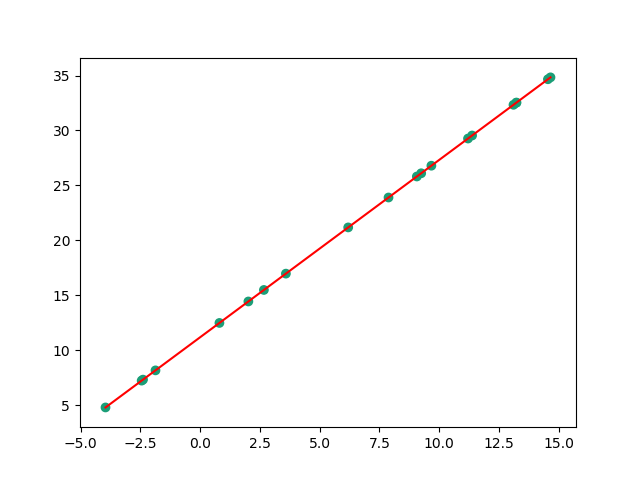
\includegraphics[width=\textwidth/3]{Figure_1}
		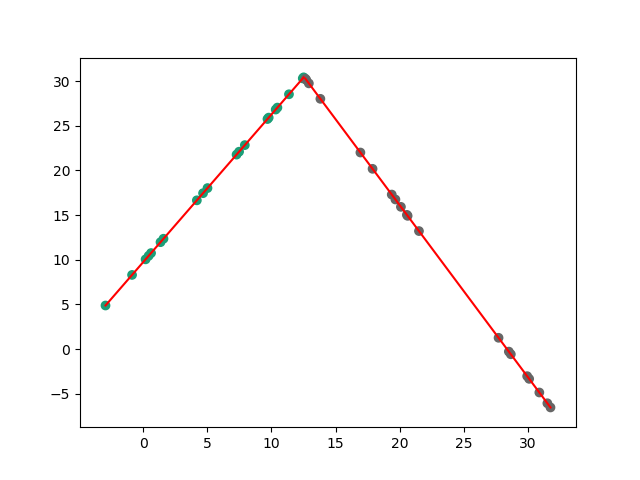
\includegraphics[width=\textwidth/3]{Figure_2}						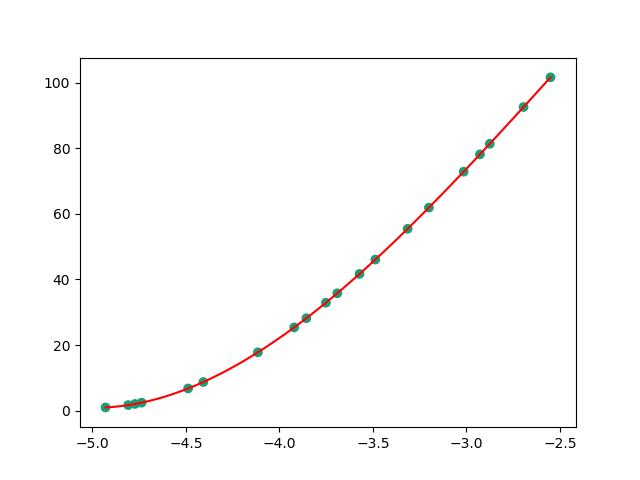
\includegraphics[width=\textwidth/3]{Figure_3}						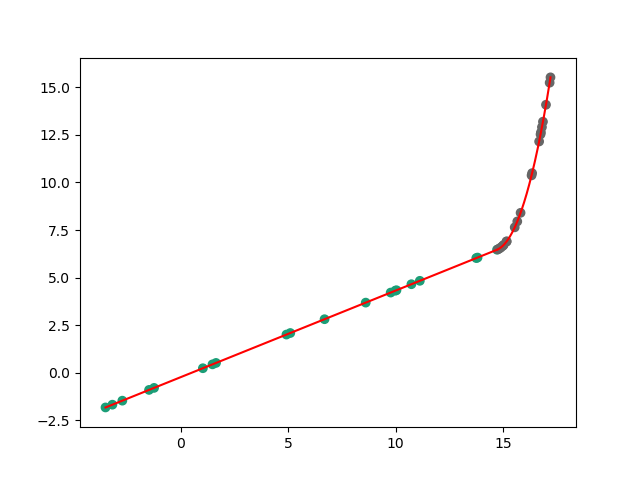
\includegraphics[width=\textwidth/3]{Figure_4}						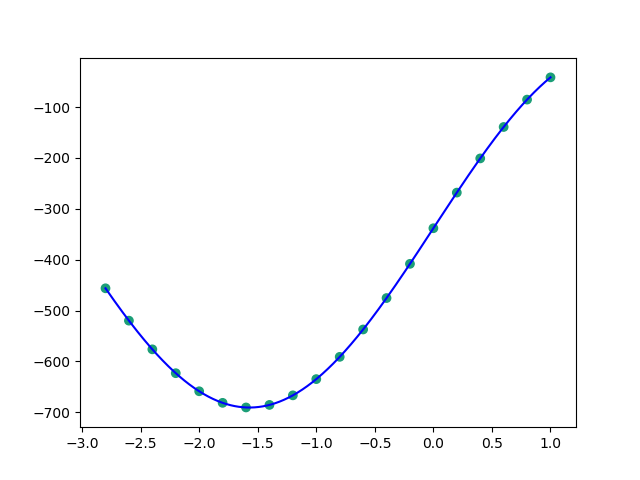
\includegraphics[width=\textwidth/3]{Figure_5}						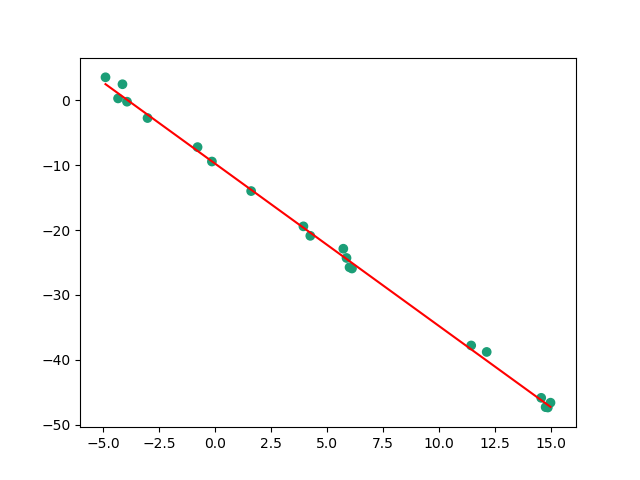
\includegraphics[width=\textwidth/3]{Figure_6}						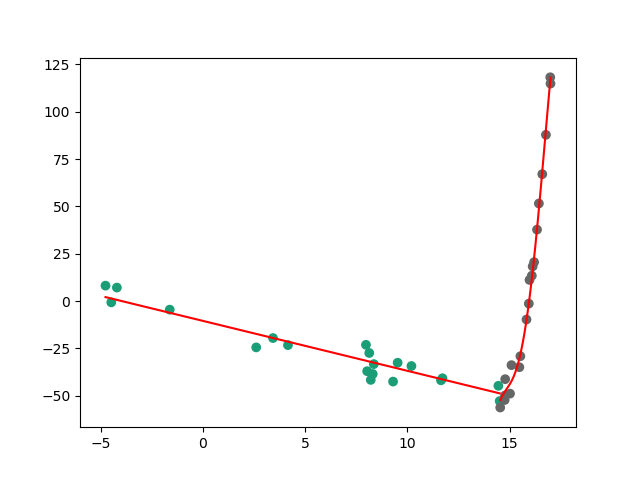
\includegraphics[width=\textwidth/3]{Figure_7}						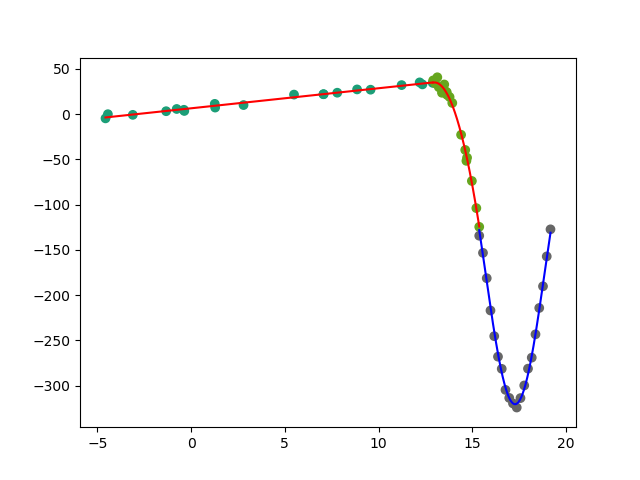
\includegraphics[width=\textwidth/3]{Figure_8}						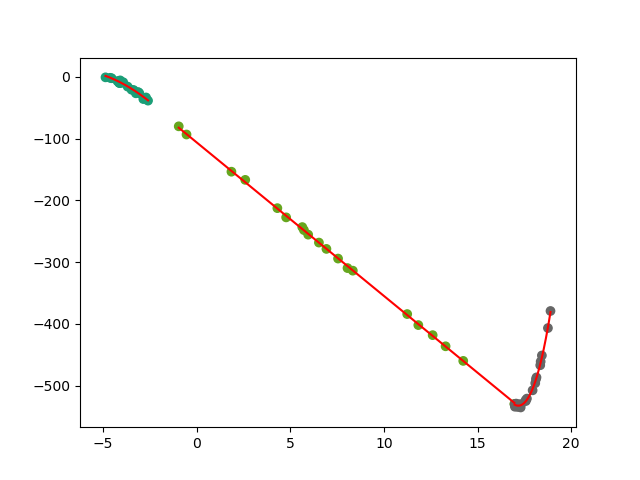
\includegraphics[width=\textwidth/3]{Figure_9}						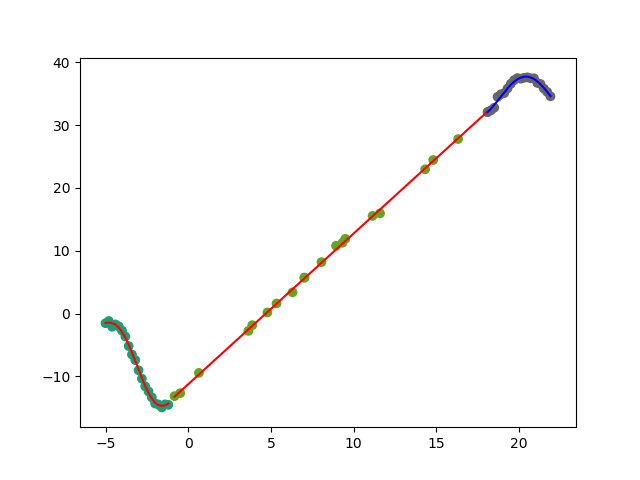
\includegraphics[width=\textwidth/3]{Figure_10}						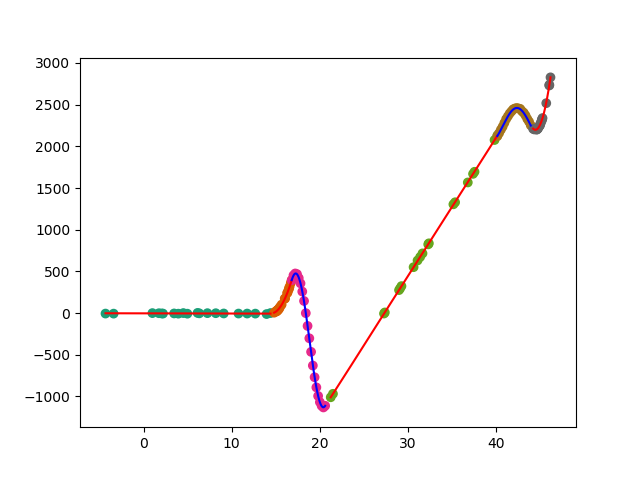
\includegraphics[width=\textwidth/3]{Figure_11}								
		\section{overfitting and new data}
				
		\section{implementation}
		
	\end{document}